%% 
%% ACS project dissertation template. 
%% 
%% Currently designed for printing two-sided, but if you prefer to 
%% print single-sided just remove ",twoside,openright" from the 
%% \documentclass[] line below. 
%%
%%
%%   SMH, May 2010. 


\documentclass[a4paper,12pt ]{report}


%%
%% EDIT THE BELOW TO CUSTOMIZE
%%

\def\authorname{Nikola Mrk\v{s}i\'c\xspace}
\def\authorcollege{Trinity College\xspace}
\def\authoremail{nm480@cam.ac.uk}
\def\dissertationtitle{{The Automated Statistician for Gaussian Process Classification}}
\def\wordcount{0}


%\usepackage{a4}
\usepackage{verbatim}
\usepackage{amsmath} 
\usepackage{amssymb,amsfonts}
\usepackage{hyperref}
\usepackage{mathtools}
\usepackage{amsthm}
\usepackage{booktabs}
\usepackage{multirow}
\usepackage{bm}
\usepackage{algpseudocode}
\usepackage{algorithm}
%\usepackage{adjustbox}
\usepackage{tocloft}
  %\usepackage[framed,numbered,autolinebreaks,useliterate]

  \usepackage{epsfig, epstopdf, graphicx,parskip,setspace,tabularx,xspace} 

\usepackage{preamble}
\usepackage{natbib}
\usepackage{color}
\usepackage{wasysym}
%\usepackage{subfigure}
\usepackage{bm}
  
  
\newtheorem{theorem}{Theorem}[section]
\newtheorem{proposition}[theorem]{Proposition}
\newtheorem{lemma}[theorem]{Lemma}
%\newtheorem{definition}[theorem]{Definition}
\newtheorem{examples}[theorem]{Examples}
\newtheorem{remarks}[theorem]{Remarks}
\newtheorem{corollary}[theorem]{Corollary}
\newtheorem{remark}[theorem]{Remark}
\newtheorem{example}[theorem]{Example}
\newtheorem{conjecture}[theorem]{Conjecture}
\newtheorem{question}[theorem]{Question}

\newcommand{\exedout}{%
  \rule{0.8\textwidth}{0.5\textwidth}%
}

\hypersetup{
    colorlinks=false,
    pdfborder={0 0 0},
}


%% START OF DOCUMENT
\begin{document}




%% FRONTMATTER (TITLE PAGE, DECLARATION, ABSTRACT, ETC) 
\pagestyle{empty}
\singlespacing
% title page information
\begin{titlepage} 

\begin{center}
\noindent
\huge
\dissertationtitle \\
\vspace*{\stretch{1}}
\end{center}

\begin{center}
\noindent
\huge
\authorname \\
\Large
\authorcollege      \\[24pt]

\includegraphics{CUni3.pdf}
\end{center}

\vspace{24pt} 

\begin{center}
\noindent
\large
{\it A dissertation submitted to the University of Cambridge \\ 
in partial 	fulfilment of the requirements for the Part III of \\ 
the Computer Science Tripos} 
\vspace*{\stretch{1}}
\end{center}

\begin{center}
\noindent
\Large \today
\end{center}



\begin{center}
\noindent
University of Cambridge \\
Computer Laboratory     \\
William Gates Building  \\
15 JJ Thomson Avenue    \\
Cambridge CB3 0FD       \\
{\sc United Kingdom}    \\
\end{center}





\end{titlepage} 

\newpage
\vspace*{\fill}

\onehalfspacing
\newpage
{\Huge \bf Declaration}

\vspace{24pt} 

I \authorname of \authorcollege, being a candidate for the Part III in
Computer Science, hereby declare that this report and the
work described in it are my own work, unaided except as may be
specified below, and that the report does not contain material that
has already been used to any substantial extent for a comparable
purpose.

\vspace{24pt}
Total word count: \wordcount

\vspace{60pt}
\textbf{Signed}: 

\vspace{12pt}
\textbf{Date}:


\vfill

This dissertation is copyright \copyright 2014 \authorname. 
\\
All trademarks used in this dissertation are hereby acknowledged.



\newpage
\vspace*{\fill}

\singlespacing
\newpage
{\Huge \bf Abstract}
\vspace{24pt}

This project was done at the Cambridge Machine Learning Group, as part of the larger effort to build an \emph{Automated Statistician}.

Given a data set, the Automated Statistician should run different methods to suggest interpretable hypotheses and the potential models to use for this data.

In this project, we have shown that automatic kernel discovery can be achieved for GP classification. We implemented a kernel structure search procedure inspired by previous work on regression by other members of the Group.

The evaluation on synthetic data sets demonstrated that the greedy procedure guided by approximate marginal likelihood can recover the underlying truth in these controlled experiments. The experiments on the four real-world biomedical data sets proved that our procedure achieves predictive performance on par with other recently proposed Bayesian models. Unlike the more complex models such as Additive GPs, our search procedure builds simple and interpretable kernels, similar to those that a human modeler might build when working on the given problem.

We have shown that the constructed kernels reveal interesting and interpretable patterns in the data. To represent these patterns, we developed functionality for visualising the posterior means of the composite kernels' components. These sets of plots correspond to the patterns identified in the data. This is the first step towards producing the automated reports for the end users, which we plan to pursue in further work.


\newpage


\vspace*{\fill}


\clearpage

\pagenumbering{roman}
\setcounter{page}{0}
\pagestyle{plain}
\tableofcontents

\clearpage

%\listoffigures
%\clearpage


%\listoftables
%\clearpage


\onehalfspacing

%% START OF MAIN TEXT 

\chapter{Introduction}
\pagenumbering{arabic} 
\setcounter{page}{1} 

\section{Bayesian Machine Learning in the context of Data Science}


%This is the introduction where you should introduce your work.  In general the thing to aim for here is to describe a little bit of the
%context for your work --- why did you do it (motivation), what was the hoped-for outcome (aims) --- as well as trying to give a brief
%overview of what you actually did.

% It's often useful to bring forward some ``highlights'' into this chapter (e.g.\ some particularly compelling results, or a particularly interesting finding). 

%It's also traditional to give an outline of the rest of the document, although without care this can appear formulaic and tedious. Your call. 

\section{Contribution}


\clearpage

%\chapter{Background} 

% A more extensive coverage of what's required to understand your work. In general you should assume the reader has a good undergraduate degree in computer science, but is not necessarily an expert in 
% the particular area you've been working on. Hence this chapter may need to summarize some ``text book'' material. 

% This is not something you'd normally require in an academic paper, and it may not be appropriate for your particular circumstances. Indeed, in some cases it's possible to cover all of the ``background'' 
%material either in the introduction or at appropriate places in the rest of the dissertation. 

\chapter{Gaussian Processes}

\section{The Role of Kernels for Gaussian Processes}

Describe different types of kernels. 

\section{Gaussian Process Classification}

Explain why it is harder, non-Gaussian likelihood...

\subsection{The Laplace Approximation to Marginal Likelihood}

\subsection{Expectation Propagation}

\subsection{Variational Bayes}

\clearpage

\chapter{Related Work} 

\section{Kernel learning}

General review of work done, with different models.

\section{Kernel structure discovery for regression}

Unsupervised structure discovery - mention that paper, maybe initially, as a similar type of work... 1 paragraph? 

Talk about the fact that these methods fix the structure of the kernel beforehand. Do they? Or they lack interpretability.


%This chapter covers relevant (and typically, recent) research which you build upon (or improve upon). There are two complementary goals for this chapter: 
%\begin{enumerate}  %  \item to show that you know and understand the state of the art; and  %  \item to put your work in context   %\end{enumerate} 

% Ideally you can tackle both together by providing a critique of related work, and describing what is insufficient (and how you do better!)

%The related work chapter should usually come either near the front or
%near the back of the dissertation. The advantage of the former is that
%you get to build the argument for why your work is important before
%presenting your solution(s) in later chapters; the advantage of the
%latter is that don't have to forward reference to your solution too
%much. The correct choice will depend on what you're writing up, and
%your own personal preference.

As a critique, discuss different information criteria, i.e. the fact that RQs can be penalised more than an SE... preferring products to additive components, say that this is something we evaluate thoroughly and try to improve on. 

Write an intro to doing this for classification, why it is harder (less information than regression, harder interpretability, non-Gaussian likelihoods and the need to resort to nlml approximations). 


\section{Additive Gaussian Processes}

Find other relevant work - Dave mentioned some of these. Read through all the papers' relevant work sections. 


\clearpage

\chapter{Kernel Structure Discovery for GP Classification} 

\section{Defining the Kernel Grammar}

Draw the basic kernels, describe additive and product kernels. 

Present challenges for classification, difference from regression, lack of clear component interpretability, as opposed to i.e. time-series data. 

\subsection{The Search Operators}

Adding or multiplying with a base kernel. 

\section{Model selection}

\section{Optimising the Hyperparameters}

Subsampling the training data to optimize the process. 

Discuss parallelisation. Maybe add a table of running times and numbers of restarts. 

\subsection{Overfitting}

Dealing with very small and very large hyperparameters. 

\section{Guiding the Structure Search}

\subsection{Bayesian and Akaike Information Criteria}

\subsection{The Number of Effective Hyperparameters}

Outline BIC light, present it as middle ground between full BIC and AIC. 
Insert the number of search steps figure that shows overfitting. 


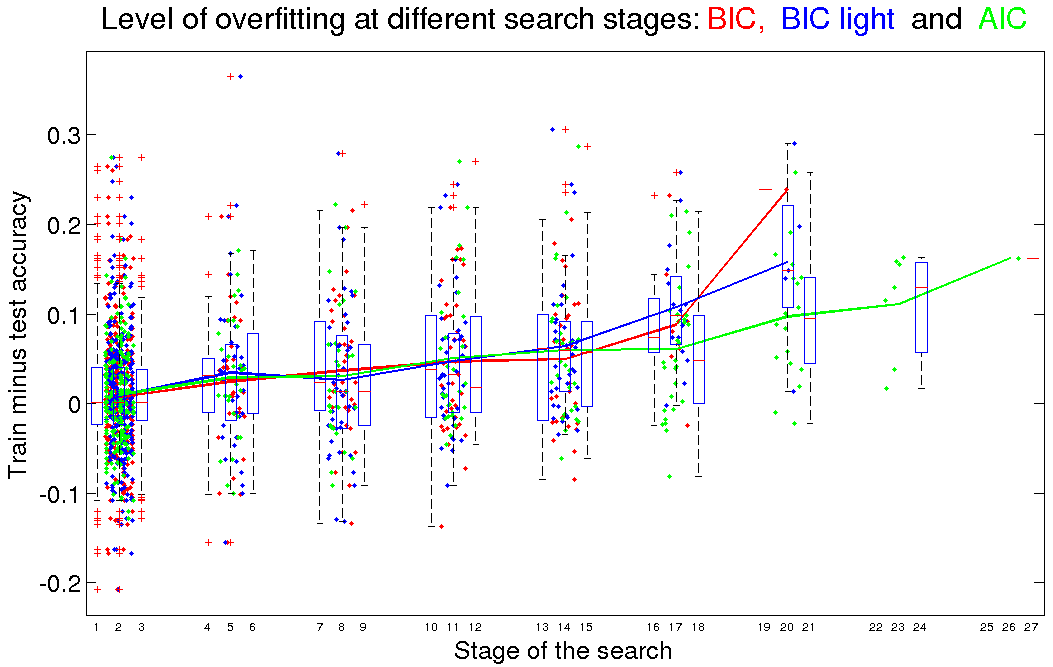
\includegraphics[scale=0.37]{figures/measureoverfit.png}

\subsection{Cross-validated training accuracy}



%\chapter{Predictive Power, Interpretability and Visualisation}

\section{Adapting the likelihood function}

\subsection{Dealing with Outliers}

a problem with classification and BIC is that estimating the number of effective hyperparameters is hard: not all of them affect the classification boundary equally. The only thing important for classification is the zero-crossings of the function (where it is greater, and where it is smaller than 0, for the purposes of prediction). Hence, smaller length-scales are the most important factor (as they determine the predictive mean and where the crossings exactly are). Larger lengthscales equate to multiplication with a constant function, so less beneficial. Signal variances are useful for computing the predictive variances, but we only care about the predictive means for determining the target label. Not counting signal frequencies might add a quick boost to quality of BIC as a model discriminator (i.e. not number of product terms, but 0 - won’t decrease by 2, but might help our choice-making). 

The reason that GPs out of the box are easily outperformed by classification specific schemes such as SVMs is that “soft-margin” SVMs are less certain of their predictions, and hence are less certain about points far away from the high density regions of the data. SVMs are never more certain than the estimated level of pepper noise (outliers in the sense of noise in the target labels of the data) whereas GPs would be very certain about points close to one of the clusters...

As a potential solution, we might want to use a @likMix which adds the “pepper noise” into the likelihood function, determining the level of the outliers and thus having the likelihood (i.e. sigmoid) which doesn’t range from 0 to 1, but from $\alpha$ to $(1 - \alpha)$, where $\alpha$ is the level of pepper noise, which is, again, to be learnt from the data? This can be implemented in GPML using @likMix, and is something we can first evaluate w.r.t. synthetic data we previously generated. The only difference is that now we add additional salt and pepper noise (random outliers) into the data and we compare performance (on this dataset) of likMix vs likErf on its own.


\section{Providing Interpretability}

\subsection{Pima}

\begin{center}

\makebox[(\textwidth) ]{
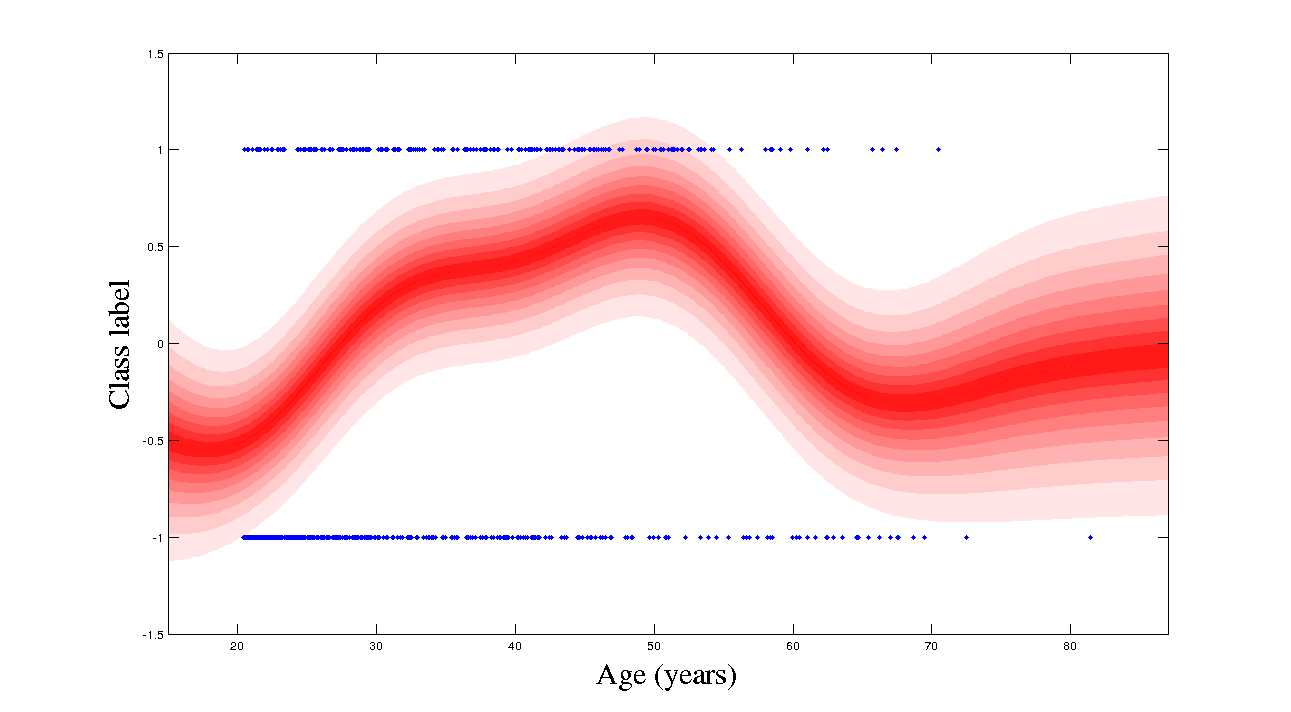
\includegraphics[trim=2cm 0cm 1cm 1cm, width=0.7\textwidth]{figures/pima/age.png}%
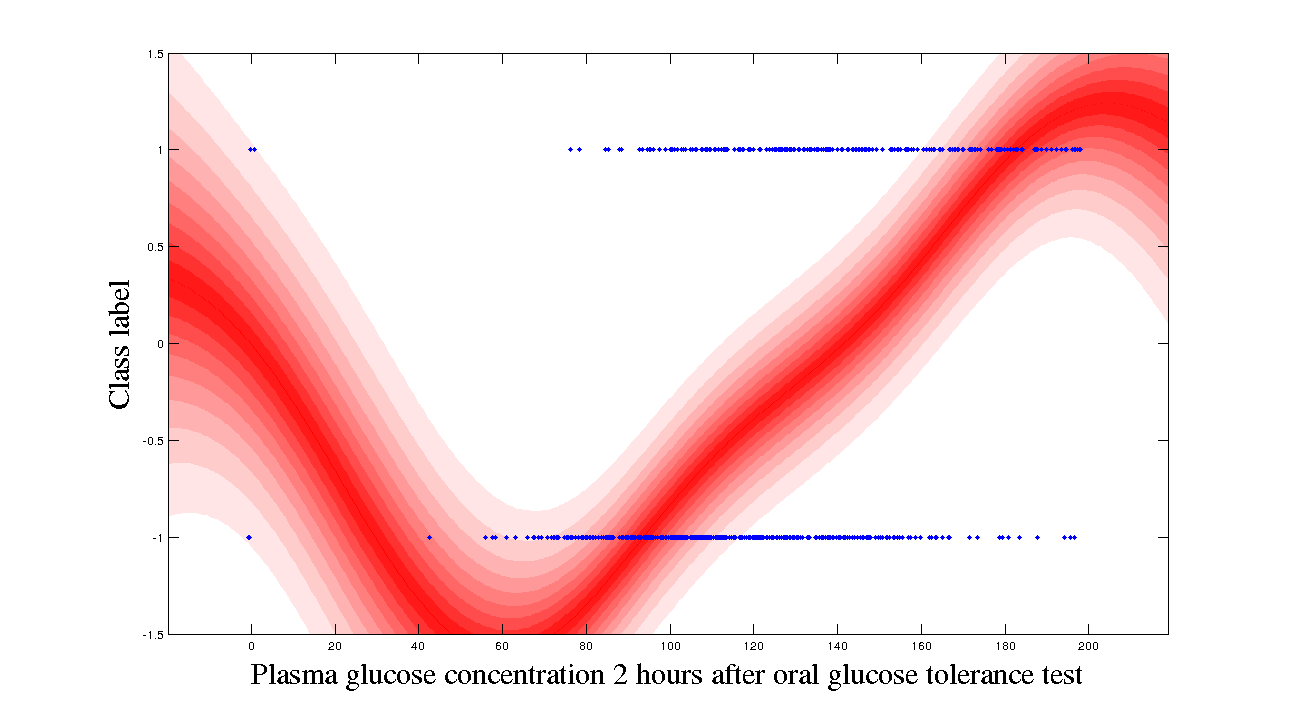
\includegraphics[trim=2cm 0cm 1cm 1cm, width=0.7\textwidth]{figures/pima/glucose.png}
}
\end{center}

\begin{center}
\makebox[(\textwidth) ]{
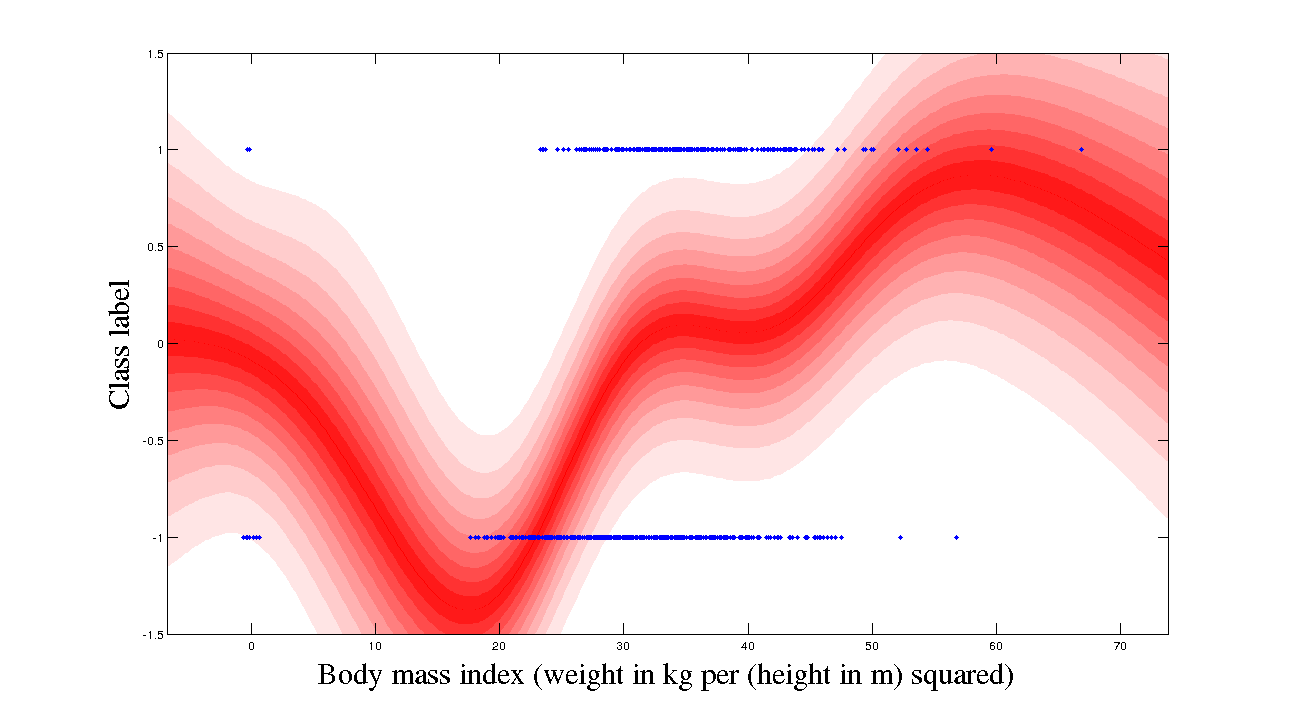
\includegraphics[trim=2cm 1cm 1cm 1cm, width=0.7\textwidth]{figures/pima/bmi.png}%
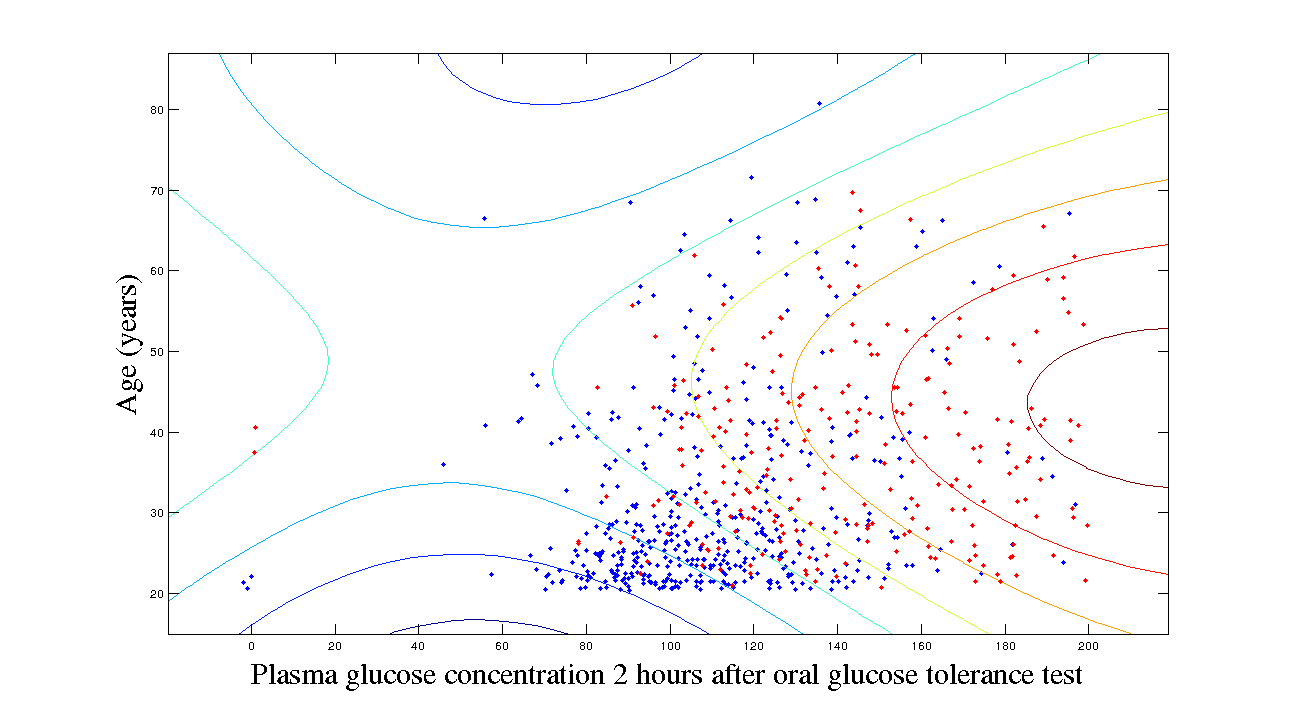
\includegraphics[trim=2cm 1cm 1cm 1cm, width=0.7\textwidth]{figures/pima/ageglucose.png}
}
\end{center}
\begin{center}


\makebox[(\textwidth) ]{
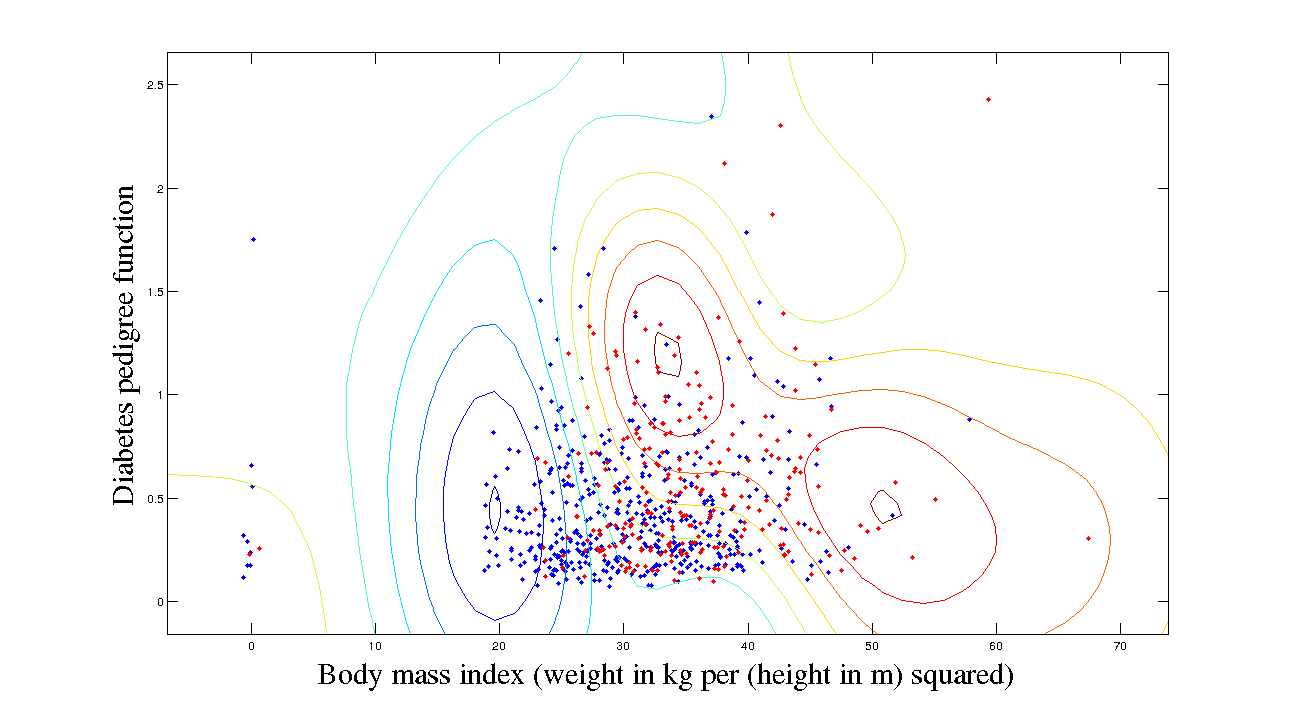
\includegraphics[trim=2cm 0cm 1cm 1cm, width=0.7\textwidth]{figures/pima/pedigreebmi.png}%
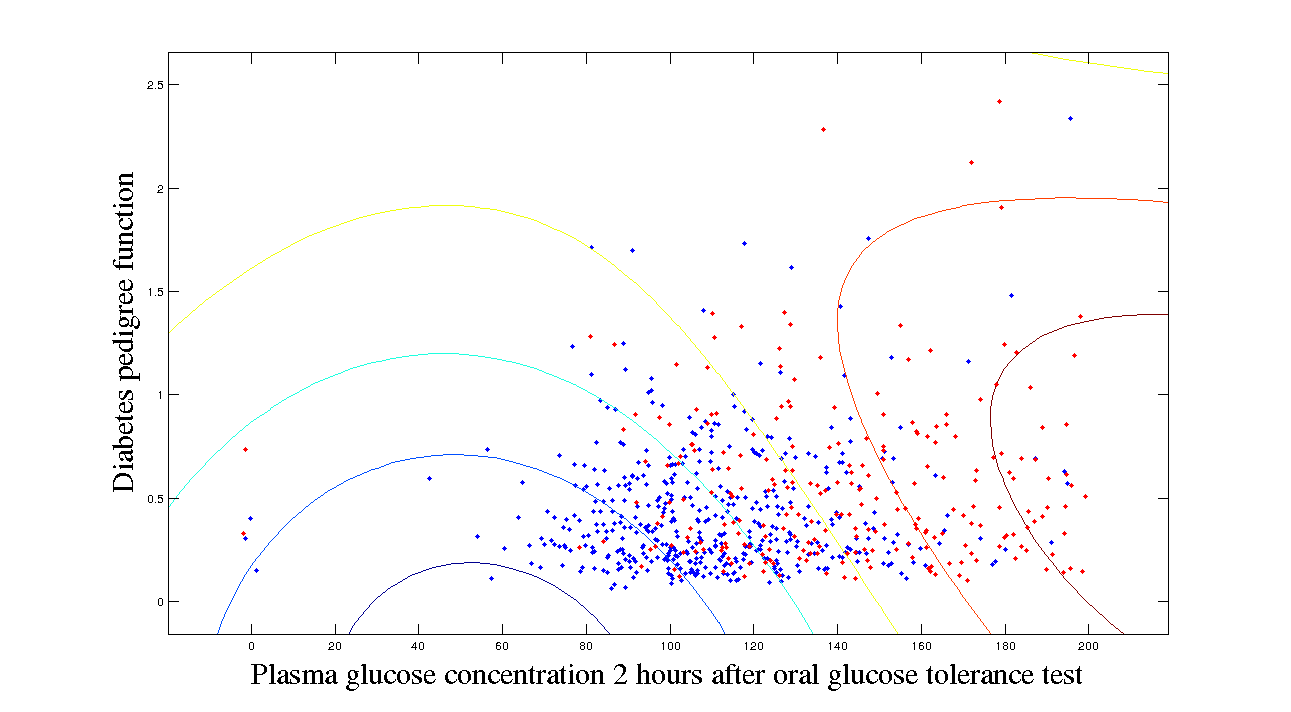
\includegraphics[trim=2cm 0cm 1cm 1cm, width=0.7\textwidth]{figures/pima/pedigreeglucose.png}
}
\end{center}

\begin{center}

\makebox[(\textwidth) ]{
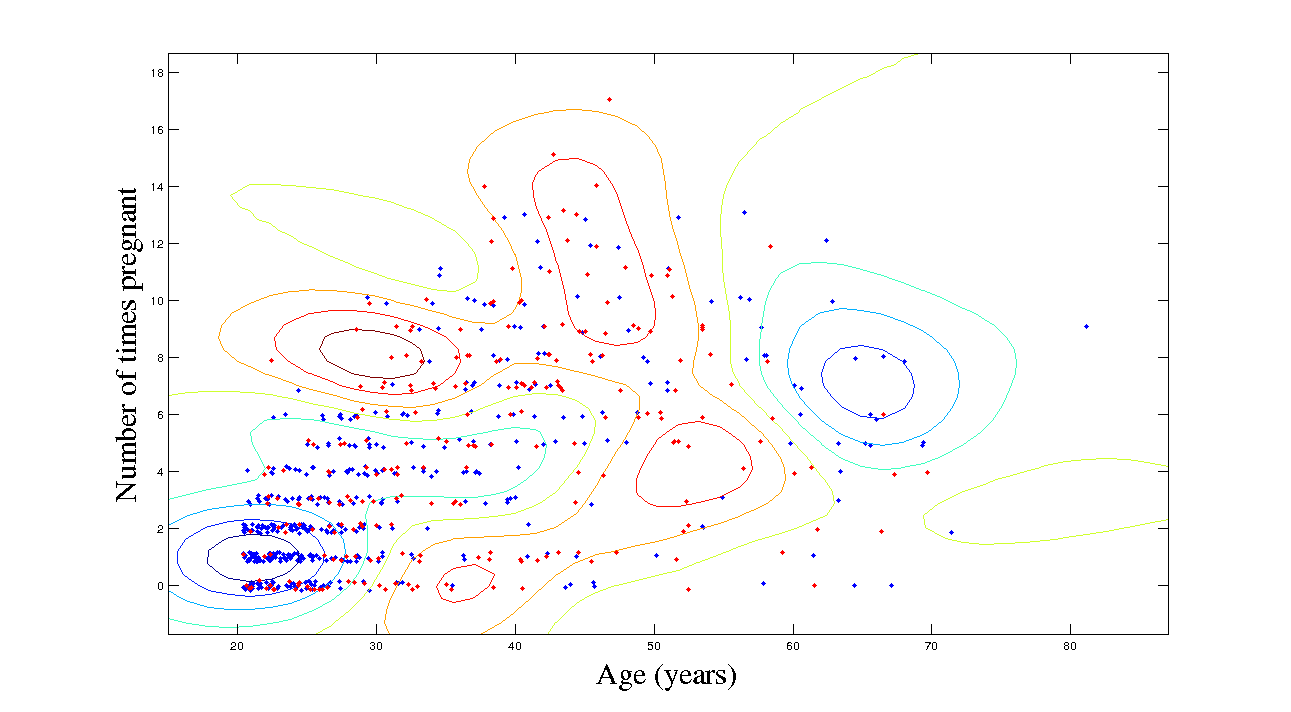
\includegraphics[trim=2cm 1cm 1cm 1cm, width=0.7\textwidth]{figures/pima/pregnantage.png}%
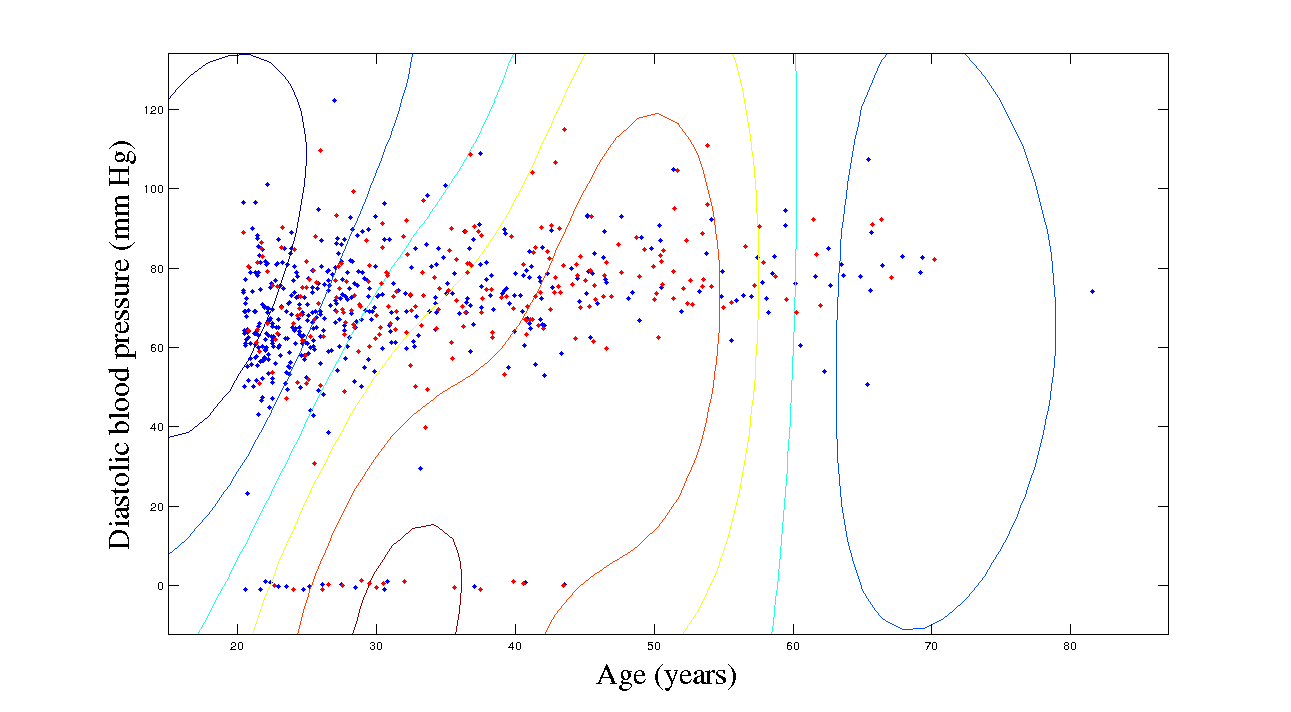
\includegraphics[trim=2cm 1cm 1cm 1cm, width=0.7\textwidth]{figures/pima/pressureage.png}
}
\end{center}

\subsection{Liver}

\subsection{Heart}


\subsection{Visualising the kernel decomposition}

\section{Bayesian Model Averaging}

\subsection{BMA for Predictive Performance}

Averaging assigned labels or probabilities converges to the same thing when many models are used. 

Discuss assigning different alphas, make a plot showing how the accuracy changes. 

\subsection{BMA for Model Selection}


\clearpage


\chapter{Evaluation} 

In this section, we consider the results achieved by the structure discovery procedure predented in the previous section. We first provide a proof of concept for the procedure by showing that it is able to extract correct kernel structure from synthetic data generated using squared
exponential kernels. We then proceed to demonstrate that the performance of the procedure on real world data sets is on par with other state of the art methods such as additive Gaussian Processes and Random Forests. Finally, we present the kernel decompositions on the real
world data sets which can be used to uncover and visualise the underlying data patterns which dictate class membership of the data points. 

\section{Experiments with Synthetic Data}

To prove that the greedy structure search procedure is able to extract structure from data, the algorithm was first applied to data drawn from a single \gp{} prior. If the BIC guiding criterion indeed picked the correct 
model based on marginal likeluihood, the procedure should be able to recover the original kernel used to generate the data. The amount of data available to the procedure, as well as the signal-to-noise ratio in the data were varied across experiments. 
As we decrease the noise levels and add more data points, the structure search should get closer to the underlying truth, that is the original kernel used to generate the data.


\begin{table}[h]

\label{tbl:synthetic}
\begin{center}

\makebox[(\textwidth) ]{

\small 
\begin{tabular}{|c |  c |  c | c | }
\hline 
{True Kernel} & { N } & { Kernel recovered (SNR = 1) } &  { Kernel recovered (SNR = 100) }  \\ \hline

&100&  $\bm{[1]}$ &$\bm{[1]}$ \\
$\bm{[1]} $ & 300& $\bm{[1]}$ &$\bm{[1]}$ \\
\emph{3 dimensions}& 500& $\bm{[1]}$ &$\bm{[1]}$ \\ \hline


&100& ${[2]}$ &${[2]}$ \\
$\bm{{[2]} + {[2]} + {[2]}} $& 300& ${[2]}$ &${[2]}$ \\
\emph{3 dimensions}& 500& ${[2]}$ &${[2]} + {[2]}$ \\ \hline


 &100& $\bm{[2\times 3]} $ &${[2]} + {[3]}$ \\
$\bm{[2\times 3]} $& 300& $\bm{[2\times 3]} $ &$\bm{[2\times 3]} $ \\
\emph{3 dimensions}& 500& $\bm{[2\times 3]} $ &$\bm{[2\times 3]} $ \\ \hline


&100& ${[4]}$ &$\bm{ {[1]} + {[2\times 3]} + {[4]} }$ \\
$ \bm { {[1]} + {[2\times 3]} + {[4]} } $ & 300& ${[2\times 3]}  + {[4]} $ &$\bm{{[1]} + {[2\times 3]} + {[4]}}$ \\
\emph{4 dimensions}& 500& $\bm{ {[1]} + {[2\times 3]} + {[4]} }$ &$ \bm{ {[1]} + {[2\times 3]} + {[4]}}$ \\ \hline


&100& ${[1]} + {[4]}$ &${[1]} + {[2]}  + {[4]}$ \\
$\bm{{[1]} + {[2\times 3]} + {[4]} }$ & 300& ${[1\times 4]} + {[2\times 3]} $  &$\bm{{[1]} + {[2\times 3]} + {[4]}}$ \\
\emph{10 dimensions}& 500& ${[1\times 4]} + {[2\times 3]} $ &$\bm{{[1]} + {[2\times 3]} + {[4]}}$ \\ \hline


 &100& ${[4]} + {[5]}$ &$ {[1\times 9]} + {[4]} $ \\
$\bm{{[1]} + {[2\times 3]} + {[5\times 6]} + {[4]} } $ & 300& ${[1]} + {[2]} + {[4]} + {[5\times 6\times 7]} $  & ${[1]} + {[1\times5\times6]}  + {[2\times3]} + {[4]}$  \\
\emph{10 dimensions}& 500& ${[1]} + {[1\times 4]} + {[2\times 3]} + {[5\times 6]} $  &${[1]} + {[1\times4\times5\times6]} + {[2\times3]} + {[4]}$  \\ \hline


&100& $\bm{{[3\times5\times7]}} $ & $\bm{{[3\times5\times7]}}$ \\
$\bm{{[3\times5\times7]}} $ & 300& $\bm{{[3\times5\times7]}}$ &$\bm{{[3\times5\times7]}}$ \\
\emph{10 dimensions}& 500& $\bm{{[3\times5\times7]}}$ &$\bm{{[3\times5\times7]}}$ \\ \hline


 &100& ${[1\times3]} + {[10]}$  &${[1\times10]} $ \\
$\bm{{[1]} + {[3\times5\times7]}  +  {[10]}} $ & 300& ${[1]} + {[10]} $ &${[1\times10]} + {[3\times5\times7]} + {[10]}$  \\
\emph{10 dimensions}& 500& ${[1]} + {[10]}$ &$\bm{{[1]} + {[3\times5\times7]} + {[10]}}$  \\ \hline


&100& ${[1]}$ &${[1]} + {[7\times9]}$ \\
$\bm{{[3\times5\times7\times9]}} $ & 300& ${[3\times5]} + {[7\times9]}$ &$\bm{{[3\times5\times7\times9]}}$ \\
\emph{10 dimensions}& 500& $\bm{{[3\times5\times7\times9]}}$ &$\bm{{[3\times5\times7\times9]}}$ \\ \hline


 &100& ${[10]}$ &${[1]} + {[3\times5\times7]}$ \\
$\bm{ {[1]} + {[3\times 5\times 7\times 9]}  + {[10]} }$  & 300& ${[1]} + {[10]}$  &${[3\times5\times7\times9]}$ \\
\emph{10 dimensions} & 500& ${[1]} + {[3\times5\times9]} + {[10]}$  & $\bm{{[1]} + {[3\times5\times7\times9]} + {[10]}}$  \\
 
\hline
\end{tabular}
}     

 \end{center}

\end{table}


Kernel optimal rates give a bound on the performance of the structure search: on average, the search is (by design) unable to construct kernels that are better than the one used to generate the data. 
The Bayes optimal rates give a theoretical limit on what any model could achieve, as they compare the actual function (y values before adding noise) to the data after the noise is added. Kernel rate should always be below the Bayes rate...

TODO: Include the same table as above with test accuracy, kernel rate, Bayes Optimal rate instead of kernel name. 


\subsection{Adding Salt and Pepper Noise}

We validated our method's ability to recover known structure on a set of synthetic datasets.
For several composite kernel expressions, we constructed synthetic data by first sampling 100, 300 and 500 points uniformly at random, then sampling function values at those points from a \gp{} prior.
We then added \iid Gaussian noise to the functions, at various signal-to-noise ratios (SNR), as well as different amounts of salt and pepper noise (random outliers in the data set). 

Table \ref{tbl:synthetic1}  lists the true kernels we used to generate the data.  Subscripts indicate which dimension each kernel was applied to.  Subsequent columns show the dimensionality $D$ of the input space, and the kernels chosen by our search for different SNRs and different amounts of added salt and pepper noise. 
We also show the kernel optimal rates (the accuracy the kernel used to generate the data achieves on the noisy test set) and the function optimal rates (the rate a classifier which knew the \emph{exact} funtion used to generate the data achieves on the noisy test data set). 



\begin{table}[h]

\caption{{ True kernel: $ \SE_1 + \SE_2 + \SE_3$, $D$ = 3.           }}

\label{tbl:synthetic1}


\begin{center}
{\small
\makebox[\textwidth]{


\begin{tabular}{|c c  c | c |  c | c c| }
\hline Data size & SNR & sp\_noise &  Kernel chosen & Test accuracy & Kernel rate & Bayes rate \\

\hline
100& 100& 0\% & $\SE_{1} + \SE_{1} \times \SE_{3} + \SE_{2}$ &87.0\% & 91.0\% & 97.4\%   \\ 
300& 100& 0\% & $\SE_{1} + \SE_{2} + \SE_{3}$ &94.0\% & 95.7\% & 97.4\%    \\
500& 100& 0\% & $\SE_{1} + \SE_{2} + \SE_{3}$ &95.8\% & 95.4\% & 97.4\%  \\  \hline
100& 100& 5\% & $\SE_{1} + \SE_{2} + \SE_{3}$ &77.0\% & 80.0\% & 91.6\%    \\
300& 100& 5\% & $\SE_{1} \times \SE_{3} + \SE_{2}$ &87.0\% & 85.7\% & 91.6\%  \\    
500& 100& 5\% & $\SE_{1} \times \SE_{2} \times \SE_{3}$ &89.8\% & 89.8\% & 91.6\%   \\  \hline
100& 100& 20\% & $\SE_{1} \times \SE_{3}$ &69.0\% & 69.0\% & 82.0\%    \\
300& 100& 20\% & $\SE_{1} \times \SE_{3} + \SE_{2}$ &75.3\% & 73.0\% & 82.0\%    \\
500& 100& 20\% & $\SE_{1} \times \SE_{3} + \SE_{2}$ &77.6\% & 74.0\% & 82.0\%   \\ \hline
100& 1& 0\% & $\SE_{1} + \SE_{3}$ &64.0\% & 72.0\% & 77.4\%    \\
300& 1& 0\% & $\SE_{1} + \SE_{3}$ &74.3\% & 75.0\% & 77.4\%    \\
500& 1& 0\% & $\SE_{1} + \SE_{3}$ &75.6\% & 76.6\% & 77.4\%  \\  \hline
100& 1& 5\% & $\SE_{1} + \SE_{3}$ &63.0\% & 63.0\% & 74.4\%    \\
300& 1& 5\% & $\SE_{1} \times \SE_{3}$ &70.7\% & 68.3\% &  74.4\%    \\
500& 1& 5\% & $\SE_{1} \times \SE_{3}$ &72.6\% & 72.6\% & 74.4\%  \\  \hline
100& 1& 20\% & $\SE_{1} \times \SE_{3}$ &53.0\% & 60.0\% & 68.8\%    \\
300& 1& 20\% & $\SE_{1} \times \SE_{3}$ &65.3\% & 65.3\% & 68.8\%    \\
500& 1& 20\% & $\SE_{1} \times \SE_{3}$ &66.2\% & 67.8\% & 68.8\%   \\
\hline

\end{tabular}
} }
\end{center}


\end{table}




\begin{table*}[h]
\caption{{ True kernel: $ \SE_1 + \SE_2 \times \SE_3 + \SE_4$,  $D$ = 4.           }}
 

\label{tbl:synthetic2}
\begin{center}
{\small
\makebox[\textwidth]{
\begin{tabular}{|c c  c | c |  c | c c| }
\hline Data size & SNR & sp\_noise &  Kernel chosen & Test accuracy & Kernel rate & Bayes rate \\

\hline
100& 100& 0\% & $\SE_{1} + \SE_{2} \times \SE_{3} + \SE_{4}$ &87.0\% & 92.0\% & 97.4\%    \\
300& 100& 0\% & $\SE_{1} + \SE_{2} \times \SE_{3} + \SE_{4}$ &94.0\% & 94.7\% & 97.4\%    \\
500& 100& 0\% & $\SE_{1} + \SE_{2} \times \SE_{3} + \SE_{4}$ &95.6\% & 96.2\% & 97.4\%    \\  \hline
100& 100& 5\% & $\SE_{1} + \SE_{2}$ &81.0\% & 76.0\% & 92.0\%    \\
300& 100& 5\% & $\SE_{1} + \SE_{2} + \SE_{3} \times \SE_{4}$ &85.7\% & 84.0\% & 92.0\%     \\
500& 100& 5\% & $\SE_{1} \times \SE_{4} + \SE_{2} \times \SE_{3} + \SE_{3}$ &87.6\% & 88.6\% & 92.0\%  \\  \hline
100& 100& 20\% & $\SE_{2} \times \SE_{4}$ &67.0\% & 67.0\% & 82.0\%    \\
300& 100& 20\% & $\SE_{2} \times \SE_{3} + \SE_{4}$ &76.0\% & 73.7\% & 82.0\%    \\
500& 100& 20\% & $\SE_{2} + \SE_{3} \times \SE_{4}$ &77.0\% & 79.8\% & 82.0\%   \\ \hline
100& 1& 0\% & $\SE_{2}$ &68.0\% & 67.0\% & 76.0\%    \\
300& 1& 0\% & $\SE_{1} + \SE_{2} \times \SE_{3}$ &72.3\% & 70.3\% & 76.0\%    \\
500& 1& 0\% & $\SE_{1} + \SE_{2} \times \SE_{3}$ &72.2\% & 73.2\% & 76.0\%  \\  \hline
100& 1& 5\% & $\SE_{2}$ &67.0\% & 58.0\% & 72.2\%    \\
300& 1& 5\% & $\SE_{1} \times \SE_{2}$ &71.0\% & 64.3\% & 72.2\%    \\
500& 1& 5\% & $\SE_{1} \times \SE_{2} \times \SE_{3}$ &70.6\% & 68.0\% & 72.2\%  \\  \hline
100& 1& 20\% & $\SE_{2}$ &59.0\% & 61.0\% & 69.0\%    \\
300& 1& 20\% & $\SE_{2} \times \SE_{3} \times \SE_{4}$ &65.3\% & 62.3\% & 69.0\%    \\
500& 1& 20\% & $\SE_{2} \times \SE_{3} \times \SE_{4}$ &64.8\% & 64.8\% & 69.0\%    \\

\hline
\end{tabular}
} }
\end{center}
\end{table*}


\begin{table*}[h]
\caption{{True kernel: $ \SE_1 + \SE_3 \times \SE_7 + \SE_{10}$,  $D$ = 10.  }} 

\label{tbl:synthetic3}
\begin{center}
{\small

\makebox[\textwidth]{

\begin{tabular}{|c c  c | c |  c | c c| }
\hline Data size & SNR & sp\_noise &  Kernel chosen & Test accuracy & Kernel rate & Bayes rate \\

\hline
100& 100& 0\% & $\SE_{1} \times \SE_{9} + \SE_{10}$ &61.0\% & 88.0\% & 96.0\%    \\
300& 100& 0\% & $\SE_{1} + \SE_{1} \times \SE_{10} + \SE_{3} \times \SE_{7}$ &92.0\% & 92.7\% & 96.0\%    \\
500& 100& 0\% & $\SE_{1} + \SE_{1} \times \SE_{3} \times \SE_{7} \times \SE_{10} + \SE_{10}$ &94.2\% & 94.6\% & 96.0\%   \\ \hline
100& 100& 5\% & $\SE_{1} \times \SE_{9} + \SE_{10}$ &53.0\% & 71.0\% & 91.8\%    \\
300& 100& 5\% & $\SE_{1} + \SE_{3} \times \SE_{7} + \SE_{6} \times \SE_{10}$ &82.0\% & 81.3\% & 91.8\%    \\
500& 100& 5\% & $\SE_{1} \times \SE_{3} \times \SE_{7} \times \SE_{10} + \SE_{10}$ &85.0\% & 86.2\% & 91.8\%   \\ \hline
100& 100& 20\% & $\SE_{1}$ &49.0\% & 64.0\% & 79.8\%    \\
300& 100& 20\% & $\SE_{1} + \SE_{10}$ &60.0\% & 70.0\% & 79.8\%    \\
500& 100& 20\% & $\SE_{1} \times \SE_{3} \times \SE_{7} \times \SE_{10}$ &74.2\% & 75.2\% & 79.8\%   \\ \hline
100& 1& 0\% & $\SE_{10}$ &59.0\% & 70.0\% & 74.4\%    \\
300& 1& 0\% & $\SE_{1} \times \SE_{3} \times \SE_{7} \times \SE_{10} + \SE_{10}$ &71.3\% & 72.7\% & 74.4\%    \\
500& 1& 0\% & $\SE_{1} \times \SE_{10} + \SE_{3} \times \SE_{7} + \SE_{9}$ & 72.0\% & 71.4\% & 74.4\%   \\ \hline
100& 1& 5\% & $\SE_{10}$ &55.0\% & 66.0\% & 71.4\%    \\
300& 1& 5\% & $\SE_{1} \times \SE_{10}$ &58.7\% & 68.7\% & 71.4\%    \\
500& 1& 5\% & $\SE_{1} + \SE_{10}$ &60.6\% & 69.4\% & 71.4\%  \\  \hline
100& 1& 20\% & $\SE_{3}$ &55.0\% & 56.0\% & 65.4\%    \\
300& 1& 20\% & $\SE_{10}$ &58.0\% & 61.7\% & 65.4\%    \\
500& 1& 20\% & $\SE_{1} \times \SE_{10}$ &58.2\% & 62.0\% & 65.4\%    \\
 

\hline
\end{tabular}
} }
\end{center}
\end{table*}




 
 
 \begin{table*}[h]
\caption{{ True kernel: $\SE_1 + \SE_3 \times \SE_5 \times \SE_7 + \SE_{9}$,  $D$ = 10. }} 

\label{tbl:synthetic4}
\begin{center}
{\small

\makebox[\textwidth]{%

\begin{tabular}{|c c  c | c |  c | c c| }
\hline Data size & SNR & sp\_noise &  Kernel chosen & Test accuracy & Kernel rate & Bayes rate \\
\hline


100& 100& 0\% & $\SE_{3} \times \SE_{5} \times \SE_{7}$ &85.0\% & 86.0\% & 97.0\%    \\
300& 100& 0\% & $\SE_{3} \times \SE_{5} \times \SE_{7} + \SE_{9}$ &93.7\% & 93.0\% & 97.0\%    \\
500& 100& 0\% & $\SE_{3} \times \SE_{5} \times \SE_{7}$ &91.4\% & 92.2\% & 97.0\%   \\ \hline
100& 100& 5\% & $\SE_{3} \times \SE_{5} \times \SE_{7}$ &78.0\% & 76.0\% & 91.6\%    \\
300& 100& 5\% & $\SE_{3} \times \SE_{5} \times \SE_{7}$ &84.0\% & 83.7\% & 91.6\%    \\
500& 100& 5\% & $\SE_{3} \times \SE_{5} \times \SE_{7}$ &86.2\% & 83.6\% & 91.6\%   \\ \hline
100& 100& 20\% & $\SE_{8}$ &49.0\% & 59.0\% & 82.0\%    \\
300& 100& 20\% & $\SE_{3} \times \SE_{5} \times \SE_{7}$ &68.3\% & 66.0\% & 82.0\%    \\
500& 100& 20\% & $\SE_{3} \times \SE_{5} \times \SE_{7}$ &72.2\% & 66.0\% & 82.0\%  \\  \hline
100& 1& 0\% & $\SE_{1} \times \SE_{3} \times \SE_{4} \times \SE_{5} + \SE_{7}$ &59.0\% & 66.0\% & 74.2\%    \\
300& 1& 0\% & $\SE_{3} \times \SE_{5} \times \SE_{7} + \SE_{9}$ &71.7\% & 72.7\% & 74.2\%    \\
500& 1& 0\% & $\SE_{1} + \SE_{3} \times \SE_{5} \times \SE_{7}$ &73.0\% & 70.6\% & 74.2\% \\   \hline
100& 1& 5\% & $\SE_{1} \times \SE_{3} \times \SE_{4} \times \SE_{5} + \SE_{7}$ &55.0\% & 62.0\% & 70.8\%    \\
300& 1& 5\% & $\SE_{3} \times \SE_{5} \times \SE_{7}$ &64.3\% & 68.7\% & 70.8\%    \\
500& 1& 5\% & $\SE_{3} \times \SE_{5} \times \SE_{7}$ &70.4\% & 67.4\% & 70.8\%   \\ \hline
100& 1& 20\% & $\SE_{3} \times \SE_{5} \times \SE_{9}$ &52.0\% & 64.0\% & 66.4\%    \\
300& 1& 20\% & $\SE_{3} \times \SE_{7} \times \SE_{8}$ &55.7\% & 61.7\% & 66.4\%    \\
500& 1& 20\% & $\SE_{3} \times \SE_{7}$ &56.4\% & 62.6\% & 66.4\%    \\


\hline
\end{tabular}
} }
\end{center}
\end{table*}
 


 \clearpage



\section{Experiments on Real World Data Sets}

In this section, we compare the performance of models constructed using our algorithm with related methods and show that the performance of our structurally simpler models is on par with more complicated models such as additive \gp{}s \cite{duvenaud2011additive11} and Hierarchical Kernel Learning. 
We also compare the performance of structure search using different information criteria (BIC, AIC, BIClight), as well as the search guided by cross-validated test accuracy. We also show the performance of the kernel using a likelihood mixture to account for outliers. 

The table below contains the mean classication error across 10 train-test splits between different methods. The best performing model is shown in bold, together with all other models that were not significantly different from it, according to the paired t-test for statistical significance. In
addition to the structure search, we show the performance of the random forest method, which constructs 1000 decision trees using the training data and then uses the mode of the classifications produced by these trees to label the test set data. This method was intended to be a \emph{ceiling}
performance for our methods, as its focus is just predictive performance: it does not contribute to interpretability or our understanding of the data set considered. 


\begin{table}[h!]
\caption{{\small
Classification Percent Error
}}
\label{tbl:Classification Percent Error}
\begin{center}
\begin{tabular}{| l | r r r r | }

\hline Method & \rotatebox{0}{ breast }  & \rotatebox{0}{ pima }  & \rotatebox{0}{ liver }  & \rotatebox{0}{ heart }  \\ \hline
Logistic Regression & $7.611$ & $24.392$  & $45.060$ & \emph{ \textbf{{16.082}}} \\
GP GAM & \emph{\textbf{5.189}} & \emph{\textbf{22.419}}  & \emph{ \textbf{29.842}} & \emph{\textbf{16.839}} \\
HKL & \emph{ \textbf{5.377}} & $24.261$  & \emph{ \textbf{27.270}} & \emph{ \textbf{18.975}} \\
GP Squared-exp & \emph{ \textbf{4.734}} & \emph{ \textbf{23.722}}  & \emph{ \textbf{31.237}} & \emph{ \textbf{20.642}} \\
GP Additive & \emph{ \textbf{5.566}} & \emph{ \textbf{23.076}}  & \emph{ \textbf{30.060}} & \emph{ \textbf{18.496}} \\ \hline \hline
GPSS (AIC) & ${ 6.430 }$ & $\mathbf{22.529}$  & $ {28.924}$ & $ 19.860 $ \\
GPSS (BIC) & $ { 5.980 }$ & ${23.440}$  & $ {37.010}$ & $ \mathbf{18.150} $ \\
GPSS (BIC light) & $ { 6.430 }$ & $\mathbf{ 22.270 }$  & $ \mathbf{27.500} $ & $ \mathbf{17.820} $ \\
GPSS (likMix) & $ \mathbf{ 11.240 }$ & $\mathbf{ 23.180 }$  & $ \mathbf{28.370} $ & $ \mathbf{16.460} $ \\
GPSS (crossValGuide) & $ \mathbf{ 5.090 }$ & ${ 23.700  }$  &  -  & $ \mathbf{17.160} $ \\ \hline
Random Forest & $ \mathbf{4.220} $ &  $ \mathbf{23.440} $ & $ \mathbf{24.030} $ &  $ \mathbf{17.130} $ \\ \hline
\end{tabular}
\end{center}
\end{table}

\section{Visualisation}

Describe what is being plotted and at what stage. 

Pima example: 



\clearpage

\chapter{Summary and Conclusions} 

%As you might imagine: summarizes the dissertation, and draws any conclusions. Depending on the length of your work, and how well you write, you may not need a summary here. 
%You will generally want to draw some conclusions, and point to potential future work. 

\section{Further Work}

\clearpage


\appendix
\singlespacing

\bibliographystyle{unsrt} 
\bibliography{refs} 

\end{document}
